\documentclass{scrartcl}

\usepackage[ngerman]{babel}
\usepackage[utf8]{inputenc}
\usepackage[T1]{fontenc}
\usepackage{graphicx}
\usepackage{amsmath}
\usepackage{chemmacros}
\usepackage{color}
\usepackage{enumitem}
\usepackage{icomma}
\usepackage{titlesec}
\usepackage{tikz}
\usepackage{adjustbox}
\usepackage{multirow}
\usepackage{upgreek}
\usepackage{url}
\usepackage{wrapfig}
\usepackage{geometry}
 \geometry{
 a4paper,
 total={170mm,250mm},
 left=20mm,
 top=20mm,
 }

\usepackage[activate={true,nocompatibility},final]{microtype} % better font-rendering
\usepackage[bitstream-charter]{mathdesign} % bitstream font
\titleformat{\section}[hang]{
	\usefont{T1}{bch}{b}{n}\selectfont} % "bch" - Bitstream Character, "b" - bold 
	{} % label
	{0em} % horizontal separation between label and title body
	{\hspace{-0.4pt}\Large \thesection\hspace{0.6em}} % code preceding the title
	[] % additional code following the title body
\titleformat{\subsection}[hang]{
	\usefont{T1}{bch}{b}{n}\selectfont}
	{}
	{0em}
	{\hspace{-0.4pt}\large \thesubsection\hspace{0.6em}}
	[]
\titleformat{\subsubsection}[hang]{
	\usefont{T1}{bch}{b}{n}\selectfont}
	{}
	{0em}
	{\hspace{-0.4pt}\thesubsubsection\hspace{0.6em}}
	[]


\chemsetup{ modules = all }
%\usepackage[version=4]{mhchem}
\chemsetup[redox]{pos=top} % oxid. numbers on top
\usepackage{chemfig}

\newlength{\drop}

\begin{document}
  \begin{titlepage}
    \drop=0.1\textheight
    \centering
    \vspace*{\baselineskip}
    \rule{\textwidth}{1.6pt}\vspace*{-\baselineskip}\vspace*{2pt}
    \rule{\textwidth}{0.4pt}\\[\baselineskip]
    {\LARGE Versuch 1--4 (BPH)\\[0.3\baselineskip] Bindungstheorie und Physikalische Eigenschaften}\\[0.2\baselineskip]
    \rule{\textwidth}{0.4pt}\vspace*{-\baselineskip}\vspace{3.2pt}
    \rule{\textwidth}{1.6pt}\\[\baselineskip]
    \scshape
    {Praktische Einführung in die Chemie\par}
    \vspace*{2\baselineskip}
    \vfill
    {\scshape Versuchstag:} \        {\large 14.06.2017}\par
  \end{titlepage}
\section{Theorieteil}
\subsection{Ionenbindung}
Ist bei den an einer Bindung beteiligten Atomen die Elektronegativitätsdifferenz hoch kommt es zu einer Ionenbindung. Dabei gibt das weniger elektronegative Atom Elektronen an das stärker elektronegative ab, wodurch \emph{Kationen} (positiv geladene Ionen) und \emph{Anionen} (negativ geladene Ionen) entstehen. Aufgrund der elektrostatischen Kraft zwischen diesen gegensätzlichen Ladungen ordnen sich die Ionen in einem \emph{Ionenkristall} regelmäßig an. Man unterscheidet dabei zwischen zwei Ordnungstypen:
\begin{enumerate}
	\item Nahordnung ist die in der lokalen Umgebung eines Ions befindliche Ordnung
	\item Fernordnung ist die Anordnung der einzelnen Nahordnungen zu einem Gitter
\end{enumerate}
\subsection{Kovalente Bindung}
Bei einer kovalenten Bindung teilen sich die Bindungspartner die Valenzelektronen meist (Ausnahmen z.B. \ch{H} und \ch{He}) so, dass jedem Atom nach der Oktettregel acht Valenzelektronen zugeordnet werden können. Bei kovalenten Bindungen zwischen Atomen gleicher Spezies spricht man von einer \emph{homolytischen} Bindung, bei unterschiedlichen, bzw. genauer Atomen unterschiedlicher Elektronegativität, von \emph{heterolytischen} Bindungen.  

Kovalente Bindungen lassen sich mit Hilfe der \emph{Valenzstrichformel} ausdrücken, z.B. \ch{H-H}, wobei Punkte für einzelne Valenzelektronen und Striche für Valenzelektronenpaare stehen.
\subsection{Intermolekulare Kräfte}
\subsubsection{Van-der-Waals-Kräfte}
Durch die „Bewegung“ der Elektronen entstehen für kurze Zeiträume Fluktuationen in der an sich gleichmäßigen Verteilung der Valenzelektronen, wodurch ein an sich unpolares Atom oder Molekül für kurze Zeit ein fluktuierendes Dipol bekommt. Dadurch kann bei einem benachbarten Atom oder Molekül ebenfalls ein temporäres Dipol induziert werden. So kann zwischen unpolaren Atomen oder Molekülen eine sehr schwache Anziehung, die mit der sechsten Potenz des Abstandes Abfällt, zustande kommen. Wegen der geringen Anziehung haben Stoffe, die aufgrund von Van-der-Waals-Kräften zusammengehalten werden, typischer Weise einen geringen Siede- und Schmelzpunkt.
\subsubsection{Dipol-Dipol Wechselwirkung}
Analog zur Van-der-Waals-Wechselwirkung zwischen unpolaren Teilchen herrscht auch zwischen Atomen oder Molekülen mit permanentem Dipol eine Wechselwirkung. Permanente Dipole haben im gegensatz zu fluktuierenden eine Ausrichtung, die stark durch die Form des Teilchens bedingt ist. Die Wechselwirkung zwischen permanenten Dipolen, auch \emph{Richteffekt} genannt, ist deutlich stärker als die Van-der-Waals-Wechselwirkung zwischen fluktuierenden, aber auch stärker temperaturabhängig. 
Eine bekannte Form der Dipol-Dipol Wechselwirkung ist die \emph{Wasserstoffbrückenbindung}, die z.B. eine wichtige Rolle beim Wasser einnimmt. Sie tritt auf, wenn Wasserstoff in die Nähe stark elektronegativer Teilchen, wie z.B. \ch{O} oder \ch{F} kommt.

\subsection{Die Molekülorbitaltheorie}
Um die Bindungsverhältnisse in kovalenten Bindungen zu beschreiben, bedient man sich der Molekülorbitaltheorie. Hierbei werden die Atomorbitale der an der Bindung beteiligten Atome gemäß LCAO-Methode (\textit{Linear Combination of Atomic Orbitals}) kombiniert. Man unterscheidet zwischen verschiedenen Arten von Bindungen.
\begin{wrapfigure}{r}{0.5\textwidth}
	\centering
\caption{Molekülschema von Sauerstoff\protect\footnotemark}
	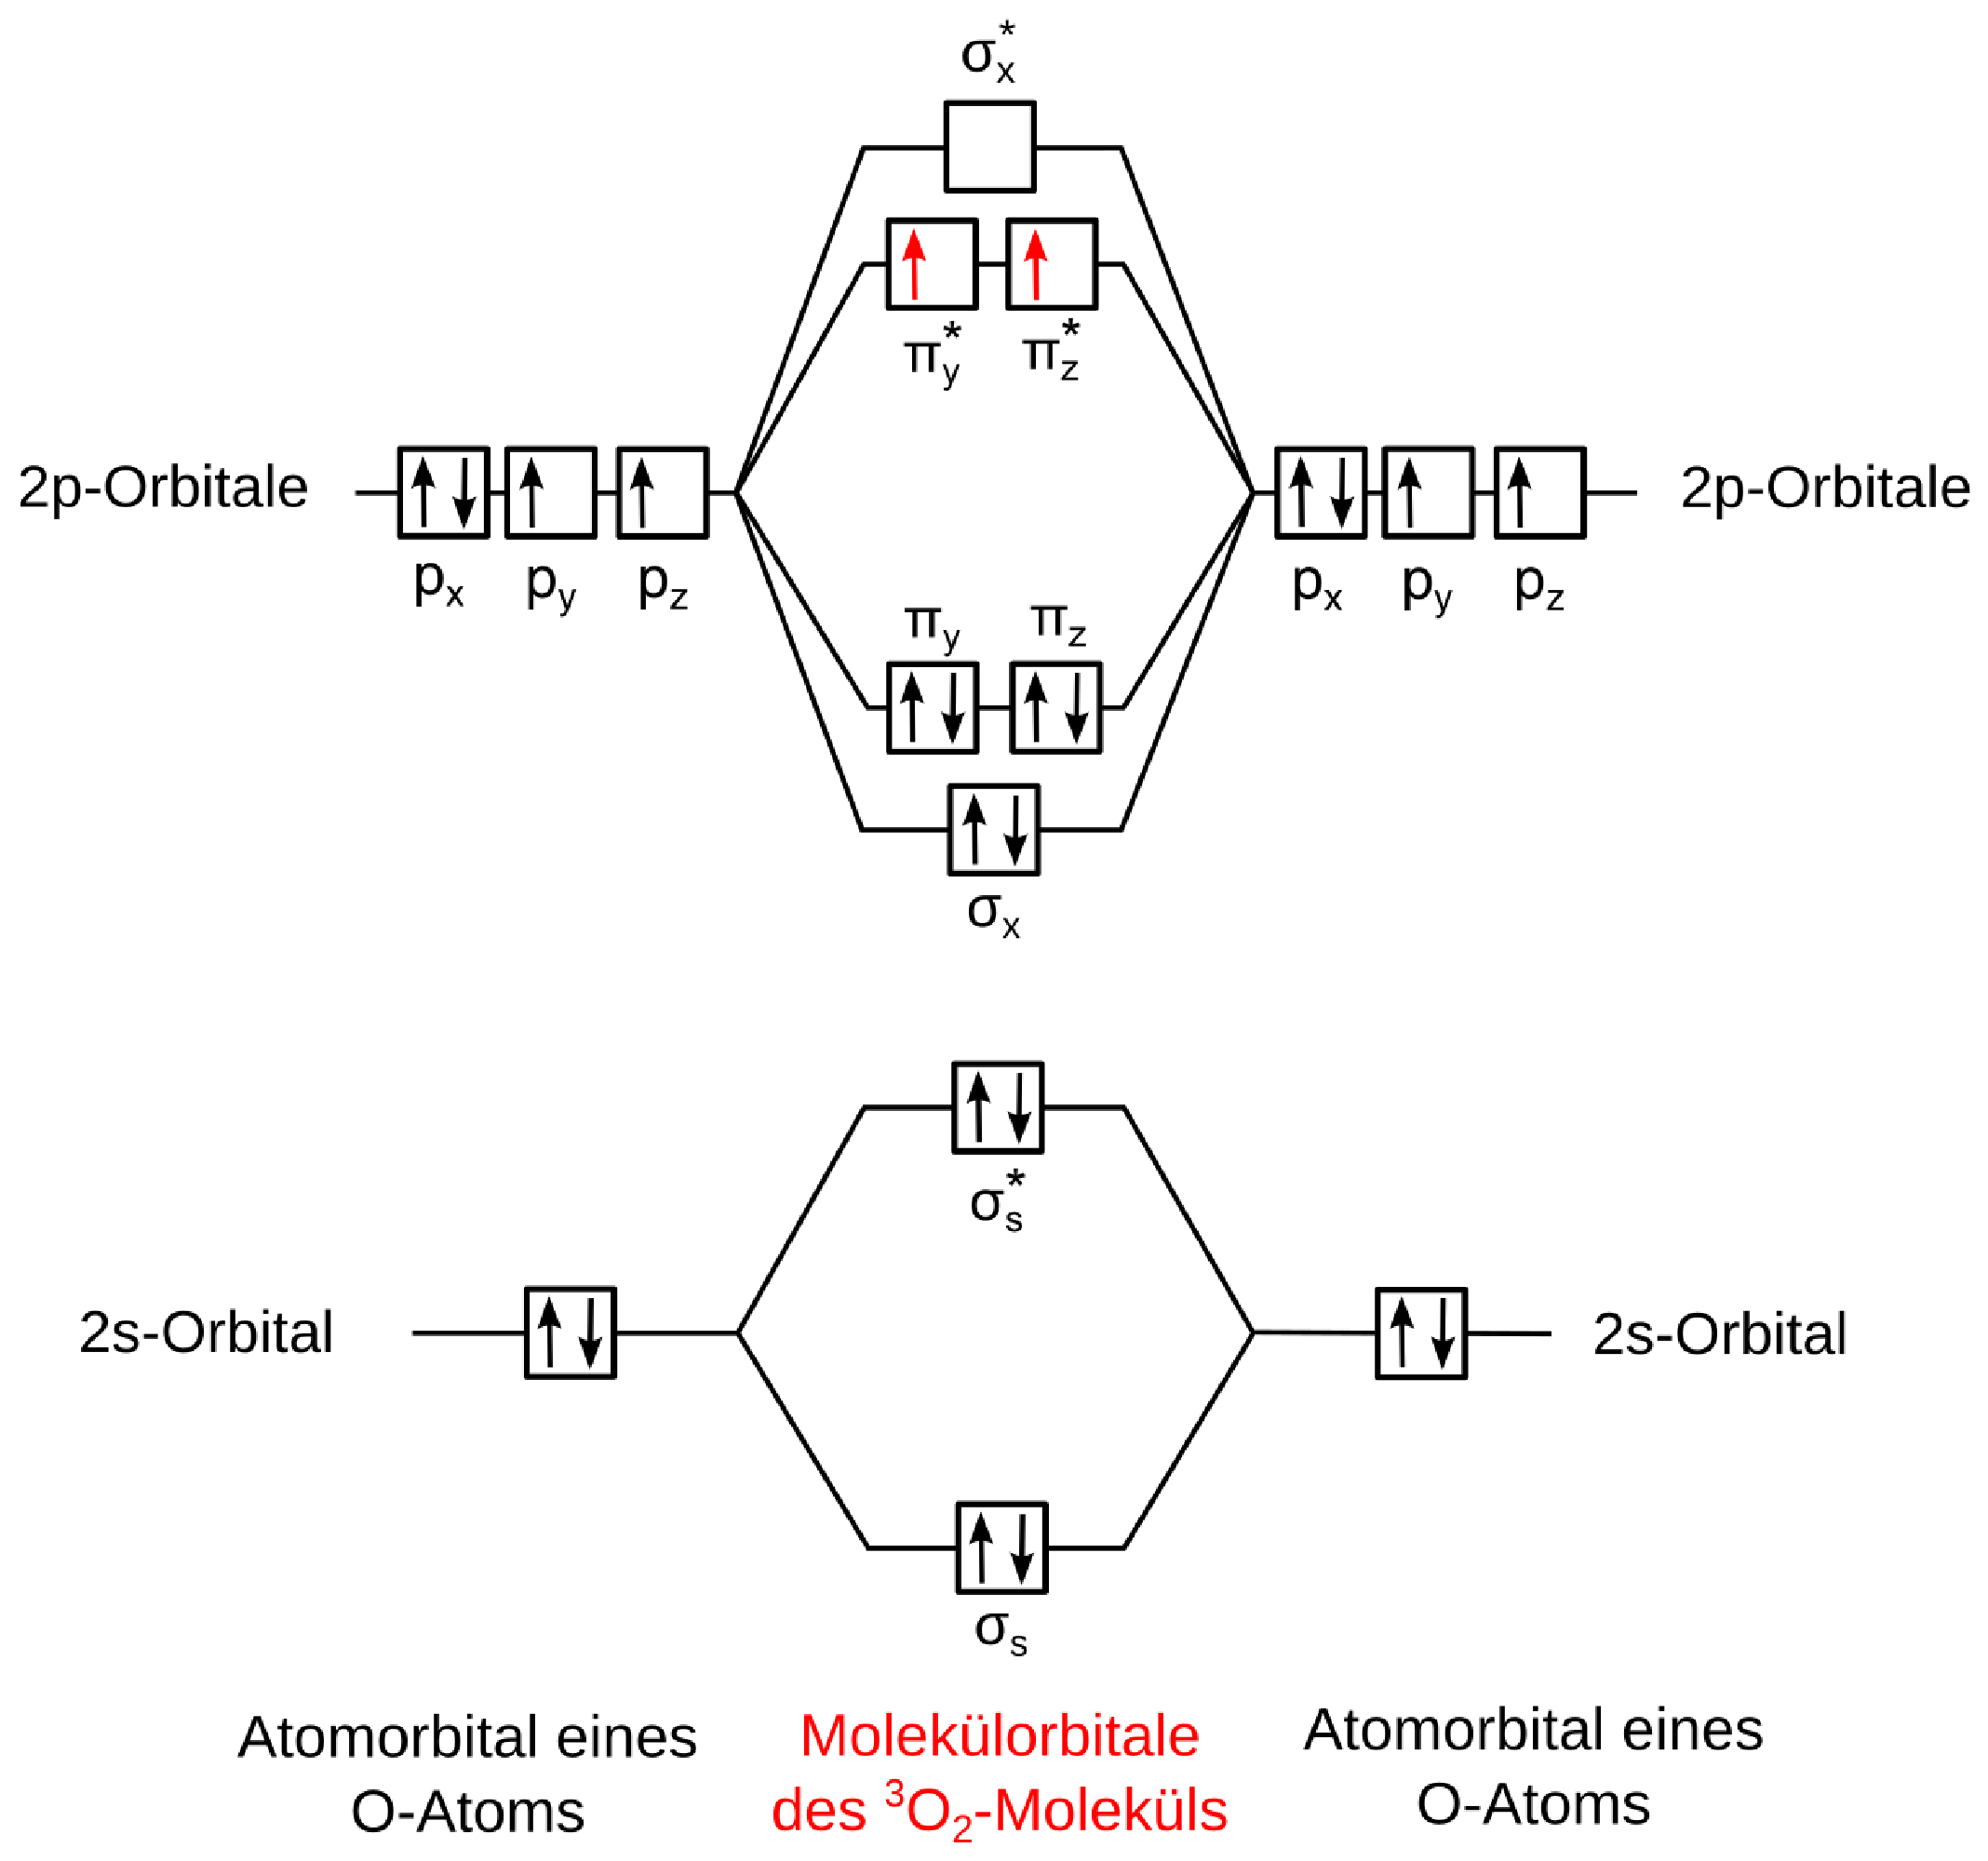
\includegraphics[width=.5\textwidth]{MO_O2.pdf}
\end{wrapfigure}
Kombiniert, bzw. überlappt man beispielsweise die Atomorbitale zweier Wasserstoffatome erhält man ein bindendes $\sigma$-Orbital. Dies entspricht der additiven oder konstruktiven Kombination der Wellenfunktionen der einzelnen Elektronen. Folglich existiert auch eine subtraktive Überlagerung geben, das sogenannte antibindende $\sigma$-Orbital, auch $\sigma^{*}$-Orbital genannt. 

Die Überlappung von $p$-Orbitalen ist etwas kompliziert als die der $s$-Orbitale. Aufgrund der räumlichen Anordnung der drei $2p$-Orbitalen entlang der $x$-, $y$- und $z$-Achse ergeben sich zum einen für die Orbitale entlang der $x$-Achse eine $\sigma$- und eine $\sigma^{*}$-Bindung, zum anderen für die Orbitale der anderen Achsen je ein $\pi$- und eine $\pi^{*}$-Bindung. Auch hier entspricht die $\pi$-Bindung einem bindenden Orbital, während $\pi^{*}$ für ein antibindendes steht. 

Zur Betrachtung der energetischen Zustände lassen sich die einzelnen Orbitale der einzelnen Atome, sowie die Orbitale der resultierenden Bindung auftragen. Bindende Orbitale sind dabei energetisch günstiger als antibindende. Die entstehenden Orbitale werden dann gemäß der \texttt{Hund'schen} Regel mit Elektronen aufgefüllt. 

\footnotetext{\url{https://commons.wikimedia.org/wiki/File:MO_Triplett_O2.svg#/media/File:MO_Triplett_O2.svg}}
Gibt es in einem Atom oder Molekül ungepaarte Elektronen, so ist der Gesamtspin des Teilchens ungleich null. Man unterscheidet folglich zwischen
\begin{itemize}
	\item \textbf{Diamagnetismus} Ein Stoff mit ausschließlich gepaarten Elektronen hat die (sehr) schwache Tendenz aus einem externen Magnetfeld herausgestoßen zu werden.
	\item \textbf{Paramagnetismus} Ein Stoff mit ungepaarten Elektronen hat die Tendenz in ein externes Magnetfeld hineingezogen zu werden. 
\end{itemize}
Ferromagneten sind Stoffe mit ungepaarten Elektronen, die nach Einfluss eines externen Magnetfeldes ihre magnetische Eigenschaft behalten, also magnetisch bleiben.

\subsection{Bändertheorie und Leitfähigkeit}
Beim Übergang von der Betrachtung einzelner Atome und Atomorbitalen zur Betrachtung mehrerer Atome und mehrerer Atomorbitalen bis hin zu denen in Festkörpern, verschmieren die klaren und diskreten Energieniveaus gewissermaßen soweit, dass man von statt von Energieniveaus der Orbitale diese als \emph{Bänder} bezeichnet. Die Valenzelektronen der Atome oder Moleküle besetzten hier das \emph{Valenzband}. Der antibindende Energiebereich wird \emph{Leitungsband} genannt. Hier können sich die Elektronen mehr oder weniger frei bewegen. Je nach dem, ob ein Bereich zwischen Valenz- und Leitungsband existiert, wird dieser \emph{Bandlücke} genannt. Nach dieser Theorie lassen sich Stoffe in drei Kategorien einteilen:
\begin{itemize}
	\item \textbf{Isolatoren} sind Stoffe, deren Valenz- und Leitungsband energetisch weit auseinander liegen, d.h. eine große Bandlücke haben. Somit können Elektronen aus dem Valenzband nur schwer in das Leitungsband überführt werden, und der Stoff leitet Strom nur sehr schlecht.
	\item \textbf{Halbleiter} sind Stoffe, bei denen zwar eine Bandlücke existiert, diese jedoch klein genug ist, dass unter Energiezufuhr die Elektronen aus dem Valenzband verhältnismäßig leicht in das Leitungsband überführt werden könnnen.
	\item \textbf{Leiter} sind Stoffe, bei denen Valenz- und Leitungsband überlappen und so die Elektronen ohne Energiezufuhr das Leitungsband besetzten. Damit leiten diese Stoffe Strom gut. 
\end{itemize}
\section{Versuche}
\subsection{Schmelzen von Salzen und Salzmischungen}
\subsubsection{Aufgabenstellung}
Es soll dokumentiert werden, wie viel Energie zum Schmelzen von Salzen und Salzmischungen nötig ist.
\subsubsection{Beobachtung}
Nach gewisser Zeit war zu beobachten, dass alle Salze (auch die Mischung) verschmolzen sind.
\subsubsection{Versuchsdurchführung}
Es wurde ein wenig von wasserfreiem \ch{Na2SO4} auf eine Magnesiarinne gegeben und dann in die wärmste Flamme des Bunzenbrenners gehalten. Dabei wurde gemessen wie viel Zeit vergangen ist bis das \ch{Na2SO4} gerschmolzen ist. Diese Vorgehensweise wurde für \ch{KNO3} und eine 1:1 Mischung aus \ch{Na2SO4 und KNO3} wiederholt. Dabei wurde nach jedem Versuch die Magnesiarinne mit demineralisiertem Wasser gesäubert um Messungenauigkeiten zu beseitigen.
\subsubsection{Versuchsauswertung}
\begin{figure}[h]
	\centering
	\caption{Schmelzzeiten der Stoffe}
\begin{tabular}{c| c c}
	Proben & Zeit [s] \\ \hline
	\ch{Na2SO4} & 48,46 \\
	\ch{KNO3} & 28\\
	Gemisch (1:1) & 69,13\\
\end{tabular}
\end{figure}
Die Tabelle zeigt wie viel Zeit vergangen ist, bis die einzelnen Proben angefangen haben zu schmelzen. Da \ch{Na2SO4} um einiges länger in seiner festen Form blieb als \ch{KNO3} ist \ch{Na2SO4} eine ionische Bindung wobei \ch{KNO3} wohl keine ionische Bindung darstellt. Wenn man die Schmelztemperaturen in Wikipedia nachschaut besitzt \ch{Na2SO4} einen Schmelzpunkt von 888$^\circ$C und \ch{KNO3} nur einen von 334$^\circ$C. Normalerweise sollte das Gemisch einen niedrigeren Schmelzpunkt besitzten als die reinen Stoffe weshalb wohl ein par Fehler unterlaufen sein müssen (siehe Fehlerbetrachtung).\\

\textbf{Eutektikum/eutektisches Gemisch:}\\
Das Eutektikum beschreibt den Punkt mit dem niedrigsten Schmelzpunkt des Gemisches. Zusätzlich zeichnet es sich aus nur sehr wenige Freiheitsgrade wählbar zu lassen. Oft wird es in einem Phasendiagramm von Temperatur auf Konzentration dargestellt(siehe Abb 1.1: Phasendiagramm). Außerdem muss ein eutektisches Gemisch nach erhitzen nicht langsam abgekühlt werden sondern kann so schnell wir möglich abgekühlt werden.
\begin{figure} 
  \centering
  \caption{Phasendiagramm\protect\footnotemark}
     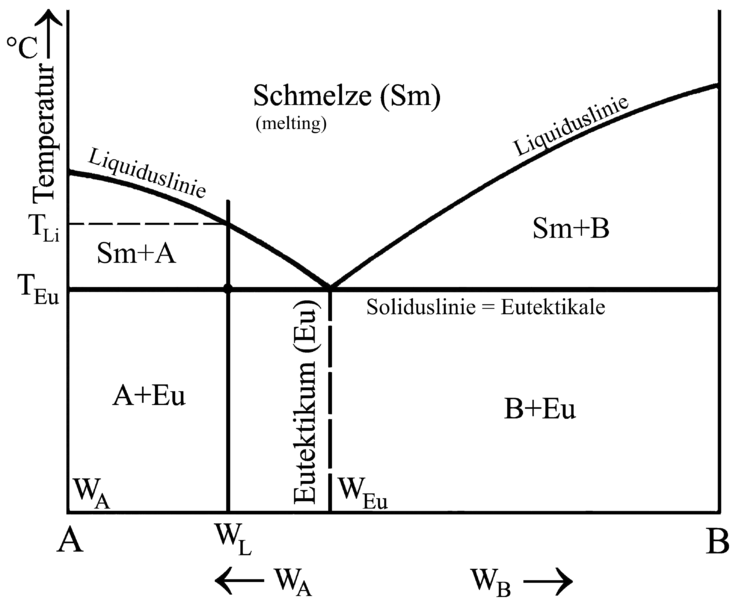
\includegraphics[width=.75\textwidth]{Phasendiagramm.png}
\end{figure}
\subsubsection{Fehlerbetrachtung}
Möglicherweise war die Mischung nicht 1:1 und somit ist nur ein kleiner Teil bei niedrigen Temperaturen geschmolzen. Dieser müsste dann so klein sein das er übersehen wurde in der Brennerflamme. Dafür müsste die Mischung jedoch stark abweichen von dem genommenen Mischungsverhältnis, sodass das eutektische Gemisch wie erwartet früh in Lösung ging, der Großteil jedoch noch reines Probematerial war und dieses natürlich länger braucht um zu schmelzen. Da jedoch die Schmelze erst 20 Sekunden nach der reinen Probe von \ch{Na2SO4} in Lösung ging muss ein anderer Fehler vorliegen. Der einzige nicht menschliche bedingter möglicher Fehler liegt darin, dass unser Gemisch aus anderen Gläsern erstellt wurde. Bei diesen wurden jedoch nach dem gleichen Verfahren die Zeit genommen bis der Schmelzpunkt erreicht war und diese lagen beide unterhalb von 25 Sekunden (bei der reinen Probe). Weshalb diese Fehlerquelle auch außer Betracht gelassen werden kann. Von daher kann es nur sein, dass starke Ungenauigkeiten beim Messen der Fall waren was möglicherweise unterstützt wurde von der schlechten Sicht auf die Probe durch die große gelbe Flamme beim im Brenner halten der Probe.
\footnotetext{\url{https://commons.wikimedia.org/wiki/File:Alloy_diagram_separate_crystal_building.png#/media/File:Alloy_diagram_separate_crystal_building.png}}

\subsection{Erhitzen, Abkühlen und Abschrecken von Schwefel}
\subsubsection{Aufgabenstellung}
Ziel war es die einzelnen Modifikationen des Schwefels beim Durchlaufen der Temperaturen von Raumtemperatur bis zum Siedepunkt und zurück zu beobachten.
Zusätzlich wurd Schwefel in seiner flüssig-plastischen Form abgeschreckt und eine Modifikation erhalten die sonst bei Standardbedigungen nicht existiert.

\subsubsection{Durchführung}
Ca. 3 g Schwefel wurden in einem Reaenzglas vorsichtig erhitzt (Brennerflamme ohne Sauerstoffzufuhr am Bunsenbrenner)(Öffnung des Reagenzglases wurde Richtung hintere Wand des Abzugs gehalten). Während dem Erhitzen wurde das Reagenzglas leicht geschwenkt um eine gleichmäßige Wärmeverteilung zu erreichen. 
Kurz vor dem Siedepunkt (zu erkennen an einer Farbänderung) wurde ein Teil der dünnflüssigen Masse in Eiwasser abgekippt (um die plastische Modifikation zu erhalten). Die noch im Reagenzglas enthaltene Masse wurde weiter erhitzt um weitere Modifikation zu erhalten. Der Bunsenbrenner wurde nun mit einer stärkeren Brennerflamme mit Sauerstoffzufuhr betrieben.

\subsubsection{Beobachtungen}
Durch das Schmelzen hat sich die Farbe von gelb zu rot-gelb geändert. Das Abschrecken im Eiswasser lies den Schwefel wieder gelb werden. Die Konsistenz war nun der von Gummi ähnlich. Weiteres Erhitzen der Flüssigkeit im Reagenzglas lies die Masse schwarz werden. Nach noch weiterem Sieden began der Inhalt des Reagenzglases zu Sieden und es bildete sich ein rötliche Niederschlag am Rand des Reagenzglases.

\subsubsection{Auswertung}
Der Ausgangsstoff (gelbes Schwefelpulver) wird als $\alpha$-Schwefel bezeichnet. Durch das Schmelzen wird dieser zu $\lambda$-Schwefel(Cyclooktaschwefel).
Wird die Flüssigkeit über 119 °C beginnt sich dieser Schwefel in Polymer-Schwefel zumzuwandeln der ab einer Temperatur von über 159 °C ausschließlich vorliegt (schwarze Flüssigkeit).
Die im Eiswasser beindliche Modifikation heißt ?.

Die Schwefelatome werden durch kovalente Bindungen zusammengehalten. Die Schwefelringe, bestehend aus jeweils 8 Schwefelatomen werden durch Van-Deer-Waals-Kräfte zusammengehalten. 

Im Versuch wurde der feste Aggregatszustand beobachtet. Durch das Schmelzen wechselte der Schwefel in den flüssigen Aggregatszustand. Nach weiterem Erhitzen wurde der Stoff verdampft bzw. wechselte in den gasförmigen Aggregatszustand.
Der Niederschlag am Reagenzglas entstand durch Resublimierung also dem direkten Übergang vom gasförmigen in den festen Aggregatszustand. Der im Eiswasser abgeschreckte Schwefel wurde erstarrt.
Die Änderung des Aggregatszustandes ist ein physikalischer Vorgang, dies liegt daran dass nur die physikalischen nicht aber die chemischen Eigenschaften des Stoffes verändert werden. Daher zählt dieser auch zu den physikalischen Eigenschaften eines Stoffes.
 
\subsection{Bestimmung der Leitfähigkeit eines metallischen Leiters}
\subsubsection{Aufgabenstellung}
Hier soll ein metallischer Leiter bei verschiedenen Temperaturen auf seinen Widerstand geprüft werden.
\subsubsection{Beobachtung}
Mit fallender Temperatur erhöht sich die Stromstärke.
\subsubsection{Versuchsdurchführung}
Ein mit Kupferdraht umwickeltes Glasrohr wurde mit zwei Klemmen befestigt und in der Mitte wurden die Sensoren des Thermometers platziert. Anschließend wurde der Kupferdraht an eine Stromquelle angeschlossen die gleichzeitig als Messgerät diente. Nun wurde der Kupferdraht mit Hilfe eines Heizföhns auf 200$^\circ$C erhitzt und es wurden jede 10$^\circ$C Messwerte notiert von der Stromstärke (die Spannung war bei dem gesamten Versuch konstant). Bei einer Temperatur von 50$^\circ$C war der Versuch beendet. 
\subsubsection{Versuchsauswertung}
\begin{figure}
	\centering
	\caption{Stromstärke und Widerstand in Abhängigkeit der Temperatur}
\begin{tabular}{l| c c c}
		Temperatur [$^\circ$C] & Stromstärke I [A] & Widerstand [R = U $\cdot$ I$\textsuperscript{-1}$ ] \\ \hline \hline
		200  & 0,825 & 1,212 \\
		190  & 0,850 & 1,176 \\
		180  & 0,835 & 1,198 \\
		170  & 0,840 & 1,190 \\
		160  & 0,845 & 1,183 \\
		150  & 0,850 & 1,176 \\
		140  & 0,855 & 1,170 \\
		130  & 0,865 & 1,156 \\
		120  & 0,870 & 1,149 \\
		110  & 0,875 & 1,143 \\
		100  & 0,870 & 1,149 \\
		 90  & 0,880 & 1,136 \\
		 80  & 0,900 & 1,111 \\
		 70  & 0,910 & 1,099 \\
		 60  & 0,920 & 1,087 \\
		 50  & 0,930 & 1,075 \\
\end{tabular}
\end{figure}
\begin{figure} 
  \centering
  \caption{Widerstand über gemessener Temperatur}
     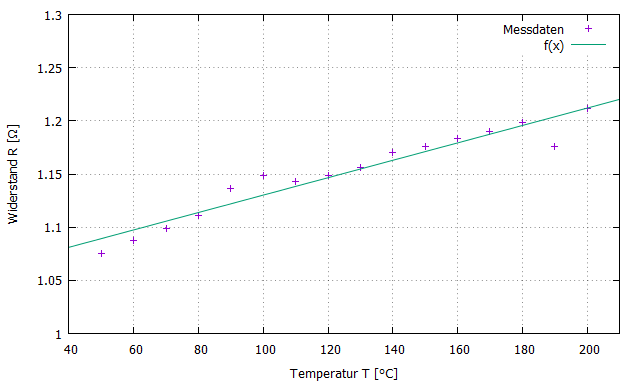
\includegraphics[width=1\textwidth]{Diagramm.png}
\end{figure}
Wenn man die Messwerte in gnuplot aufträgt sieht man, dass der Widerstandverlauf einen linearen Verlauf an nimmt, weshalb mit f(T)= a$\cdot$T+b gefittet wurde. Dabei ergibt sich eine Regressionskurve von R(T)=0.000818235$\cdot$T+1.04835.

\subsection{Magnetismus}
\subsubsection{Aufgabenstellung}
Der Versuch sollte das magnetische Verhalten eines Gadoliniumstabes in Abhängigkeit zur Temperatur dokumentieren.

\subsubsection{Versuchsdurchführung}
Am Ende eines Gadoliniumstabes wurden Permanentmagnete angebracht. Anschließend wurde das Verhalten von Eisenspähnen in einer Plastiktüte beobachtet bzw. ob diese auf ein etwaiges Magnetfeld reageieren. Dies wurde für Raumtemperatur, handwarme und in Eiswasser gekühlte Temperatur durchgeführt.

\subsubsection{Beobachtungen}
Bei Raumtemperatur war keine Bewegung der Eisenspähne zu beobachten, als der Gadoliniumstab an dem Gefäß vorbeigeführt wurde. Durch den in Eiswasser gekühlten Stab konnten die Eisenspähne etwas bewegt werden. Nach dem Wiederaufwärmen in der Hand war wiederum keine Bewegung erkennbar.
\subsubsection{Versuchsauswertung}
Manche ferromagnetischer Stoff verlieren oberhalb einer bestimmten Temperatur diese Eigenschaft. Diese Temperatur wird Curie-Temperatur genannt und liegt bei Gadolinium bei 292,5 K bzw. 19,35 °C.
 
 
\section{Literatur}
\begin{enumerate}[label=(\arabic*)]
	\item \emph{Praktische Einführung in die Chemie
für Studierende der Fachrichtungen
Technische Biologie und Physik}. Praktikumsskript, Universität Stuttgart,
SoSe 2017.  
	\item Prof. Dr. D. Gudat. \emph{„Einführung in die Chemie für Naturwissenschaftler“}. Vorlesungsskript
	\item \emph{Das Basiswissen der Chemie}. Charles E. Mortimer, Ulrich Müller. 12. Auflage
\end{enumerate}
\end{document}		
